\documentclass{article}
\usepackage{listings}
\usepackage{xcolor}
\usepackage[margin=1in]{geometry}
\usepackage{amsmath,amsthm,amssymb}
\usepackage{graphicx}
\usepackage{epstopdf}
\DeclareGraphicsExtensions{.eps,.ps,.jpg,.bmp}
\lstset{
	numbers=left,
    framexleftmargin=10mm,
    frame=none,
    backgroundcolor=\color[RGB]{245,245,244},
	keywordstyle=\bf\color{blue},
	identifierstyle=\bf,
	numberstyle=\color[RGB]{0,192,192},
	commentstyle=\it\color[RGB]{0,96,96},
	stringstyle=\rmfamily\slshape\color[RGB]{128,0,0},
	showstringspaces=false
    }

\newcommand{\N}{\mathbb{N}}
\newcommand{\R}{\mathbb{R}}
\newcommand{\Z}{\mathbb{Z}}
\newcommand{\Q}{\mathbb{Q}}

\newenvironment{theorem}[2][Theorem]{\begin{trivlist}
\item[\hskip \labelsep {\bfseries #1}\hskip \labelsep {\bfseries #2.}]}{\end{trivlist}}
\newenvironment{lemma}[2][Lemma]{\begin{trivlist}
\item[\hskip \labelsep {\bfseries #1}\hskip \labelsep {\bfseries #2.}]}{\end{trivlist}}
\newenvironment{exercise}[2][Exercise]{\begin{trivlist}
\item[\hskip \labelsep {\bfseries #1}\hskip \labelsep {\bfseries #2.}]}{\end{trivlist}}
\newenvironment{problem}[2][Problem]{\begin{trivlist}
\item[\hskip \labelsep {\bfseries #1}\hskip \labelsep {\bfseries #2.}]}{\end{trivlist}}
\newenvironment{question}[2][Question]{\begin{trivlist}
\item[\hskip \labelsep {\bfseries #1}\hskip \labelsep {\bfseries #2.}]}{\end{trivlist}}
\newenvironment{corollary}[2][Corollary]{\begin{trivlist}
\item[\hskip \labelsep {\bfseries #1}\hskip \labelsep {\bfseries #2.}]}{\end{trivlist}}

\begin{document}

\title{Homework 3}
\author{Chuan Lu\\
13300180056}

\maketitle

\begin{problem}{1}
\text{ }\\
Generate the following distribution in two ways:
$$P(x=i) = \frac{e^{-\lambda}\lambda^{i}/i!}{\Sigma_{j=0}^{k}e^{-\lambda}\lambda^{j}/j!}, i=0,\cdots, k$$
\end{problem}

\begin{proof}
\subsection{Method 1: The Inverse Transform Method}
1. Generate a random number U which is uniformly distributed over (0, 1). \\
2. Let $q_{i} = e^{-\lambda}\lambda^{i}/i!, (i=0,\cdots, k)$, $p_{i} = \frac{q_{i}}{\Sigma_{j=0}^{k}q_{i}}.$ \\
3. For i in $0, 1, \cdots, k, sum = \Sigma_{j=0}^{i}$. If $U < sum$, then set $X = i$, return. \\

% In a optimized calculating order, this method should behave like this: \\
% 1': Generate a random number U which is uniformly distributed over (0, 1).
% 2': Let $i = 0, p = e^{-\lambda}, F = p$. \\
% 3': For i in range(k) \\
% \quad 1) if $U < F$, set $X = i$, RETURN. \\
% \quad 2) $p = \lambda * p/(i+1), F = F+p, i = i+1.$

\subsection{Method 2: The Acceptance-Rejection Method}
-1: Calculate $P(x=i)$, $sum = \Sigma_{i=0}^{k}P(x=i)$, $p_{i} = P(x=i)/sum$. \\
0. While True:
1. Generate a discrete random variable Y, with a probability mass function ${q_{j} = \frac{1}{q+1}}.$ \\
\quad 1.1 Generate a random number Z which is uniformly distributed over (0, 1). \\
\quad 1.2 Return $floor(Z * (k+1))$. \\
2. Let $t = floor(\lambda-1), c = (k+1)*p_{t}.$\\
2.1 Because $\lambda < 1$, then t = 0. \\
3. Generate a random number U which is uniformly distributed over (0, 1). \\
4. If $U < (k+1)/c*p_{Y}$, set X=Y and RETURN.

\subsection{The Numerical Experiment}
\subsubsection{The code is shown as follows}
\begin{lstlisting}[language = {R}]
# Problem 1.1
p11 = function(a, lambda, k) {
  # The following functions have the same comments.
  # Generate a matrix A of random variables;
  # The number of rows and columns of A is a[1] and a[2];
  # lambda and k are the parameters in the distributional function;
  q = matrix(rep(0, k+1), nrow = 1)
  qsum = matrix(rep(0, k+1), nrow = 1)
  q0 = exp(-lambda)
  qsum0 = 0
  for(i in 1:(k+1)) {
    q[i] = q0
    qsum0 = qsum0 + q0
    qsum[i] = qsum0
    q0 = q0 * lambda / i
  }
  q = q / rowSums(q)
  qsum = qsum / qsum[k+1]
  A = matrix(rep(0, a[1] * a[2]), ncol = a[2])
  U = matrix(runif(a[1] * a[2]), ncol = a[2])
  for (i in 1:a[1]) {
    for (j in 1:a[2]) {
      place = which(U[i, j] < qsum)
      A[i, j] = place[1] - 1
    }
  }
  return(A)
}

# Problem 1.2
p12 = function(a, lambda, k) {
  q0 = exp(-lambda)
  q = matrix(rep(0, k+1), nrow = 1)
  for(i in 1:(k+1)) {
    q[i] = q0
    q0 = q0*lambda/i
  }
  q = q/rowSums(q)
  A = matrix(rep(0, a[1]*a[2]), ncol = a[2])
  for(i in 1:a[1]) {
    for(j in 1:a[2]) {
      while(1) {
        z = runif(1)
        y = floor(z*(k+1))
        c = (k+1) * q[1]
        u = runif(1)
        if (u < (k+1)/c*q[y+1]) {
          A[i, j] = y
          break
        }
      }
    }
  }
  return(A)
% }
\end{lstlisting}
\begin{lstlisting}[language = {R}]
source("main.R")

# Problem 1.1
lambda = 0.5
k = 4
a = matrix(c(1, 10000))
r1 = p11(a, lambda, k)
hist(r1)

# Problem 1.2
r2 = p12(a, lambda, k)
hist(r2)
\end{lstlisting}
\subsubsection{The result is shown as follows}
\begin{figure}[htbp]
\centering
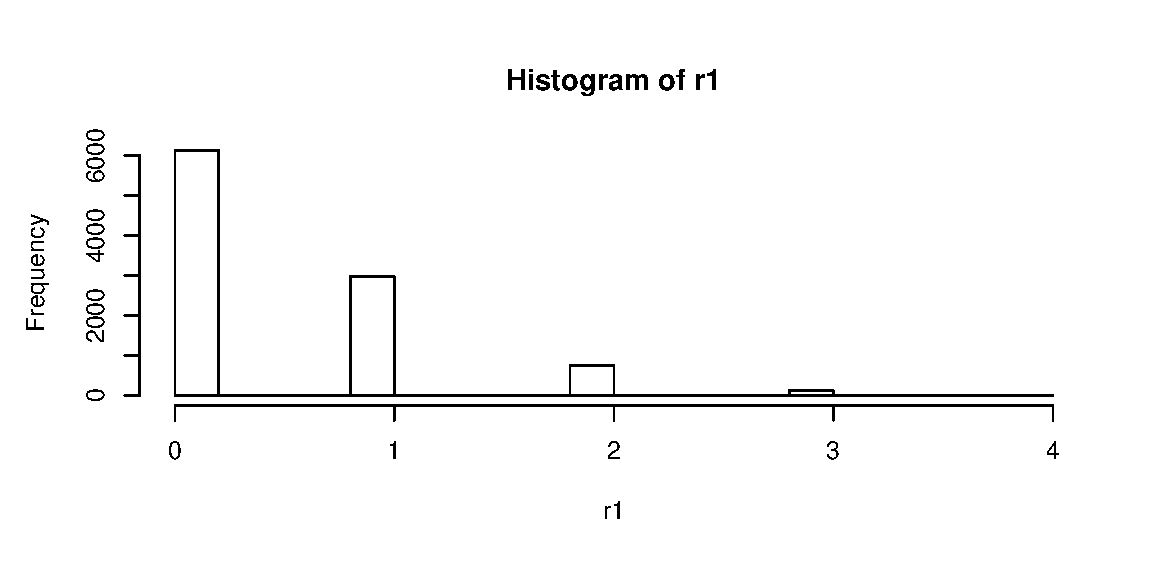
\includegraphics[width = 15cm]{r11.eps}
\caption{The numerical exp. of p1. method 1.}
\label{p1m1}
\end{figure}
\begin{figure}[htbp]
\centering
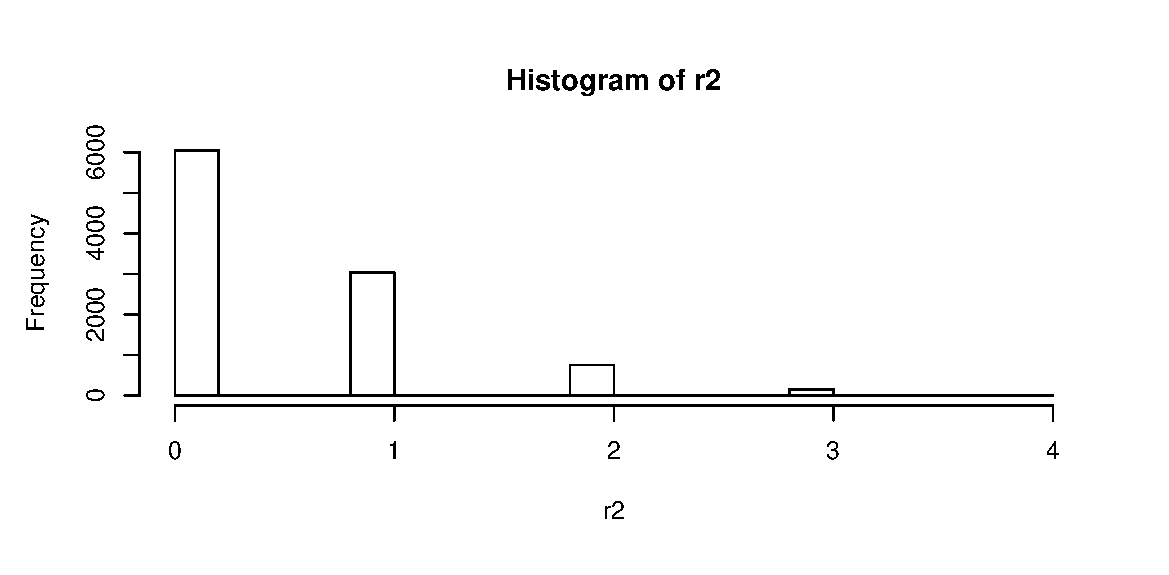
\includegraphics[width = 15cm]{r12.eps}
\caption{The numerical exp. of p1. method 2.}
\label{p1m2}
\end{figure}
\end{proof}


\begin{problem}{2}
\text{ }\\
Generate a random variable with a distribution given.
\end{problem}
\begin{proof}
\subsection{The method is given as follows}
1. Generate a random variable U which is uniformly distributed over (0, 1). \\
2. If $U < 0.55$, let $t = floor(U/0.11)$, RETURN $2*t+5$. \\
3. Else let $t = floor((U-0.55)/0.09)$, RETURN $2*t+6$. \\

\subsection{The Numerical Experiment}
\subsubsection{The code is shown as follows}
\begin{lstlisting}[language = {R}]
# Problem 2
p2 = function(a) {
  handle_func = function(u) {
    if(u < 0.55) {
      return(2*floor(u/0.11)+5)
    }
    else {
      return(2*floor((u-0.55)/0.09)+6)
    }
  }
  f = Vectorize(handle_func)
  A = matrix(runif(a[1] * a[2]), ncol = a[2])
  return(f(A))
}

# Problem 2
r3 = p2(a)
hist(r3)
\end{lstlisting}
\subsubsection{The result is shown as follows}
\begin{figure}[htbp]
\centering
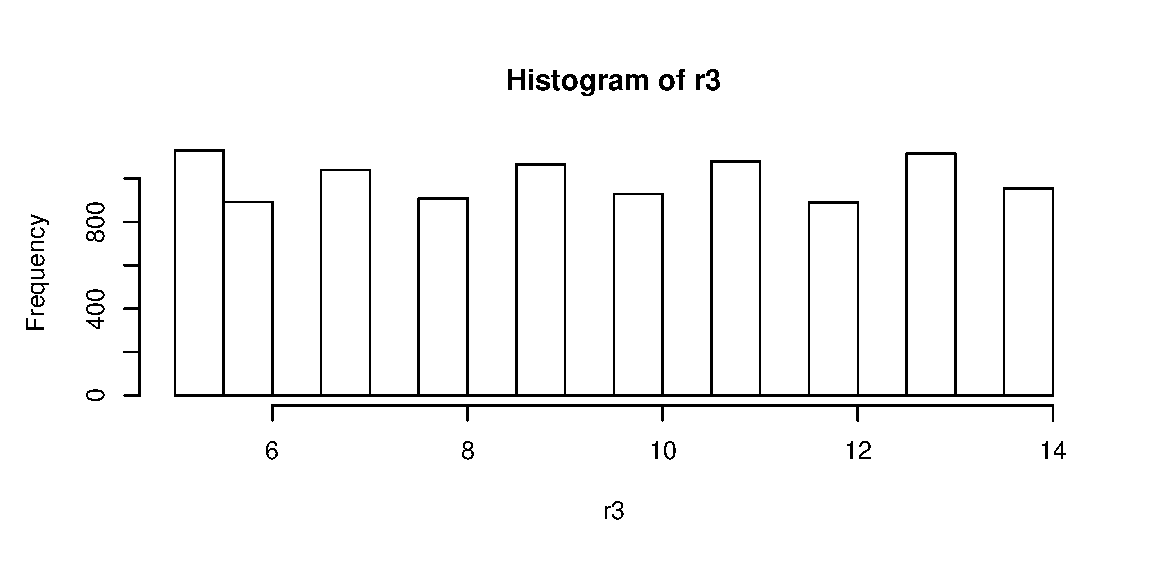
\includegraphics[width = 15cm]{r3.eps}
\caption{The numerical exp. of p2.}
\label{p2}
\end{figure}
\end{proof}


\begin{problem}{3}
\text{ } \\
Generate a continouous random variable with a distribution given.
\end{problem}
\begin{proof}
\subsection{The method is given as follows}
1. Generate two random variables U and V, which are both uniformly distributed over (0, 1). \\
2. Let $t = \frac{1}{2}log(U).$
3. If $V < 0.5$, RETURN t, else RETURN -t.

\subsection{The Numerical Experiment}
\subsubsection{The code is shown as follows}
\begin{lstlisting}[language = {R}]
# Problem 3
p3 = function(a) {
  A = matrix(runif(a[1] * a[2]), ncol = a[2])
  t = 0.5 * log(A)
  v = matrix(runif(a[1] * a[2]), ncol = a[2])
  change_place = which(v >= 0.5)
  t[change_place] = -t[change_place]
  return(t)
}

# Problem 3
r3 = p3(a)
hist(r3)
\end{lstlisting}
\subsubsection{The result is shown as follows}
\begin{figure}[htbp]
\centering
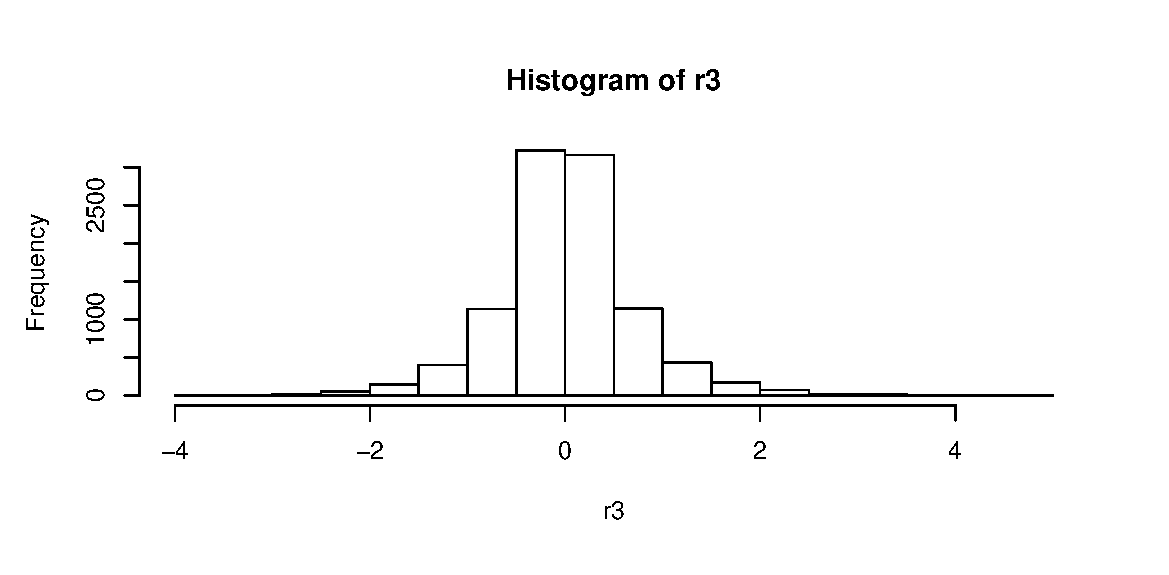
\includegraphics[width = 15cm]{r33.eps}
\caption{The numerical exp. of p3.}
\label{p3}
\end{figure}
\end{proof}

\begin{problem}{4}
\text{ }\\
Generate a random variable with the distribution given.
\end{problem}
\begin{proof}
\subsection{Use the rejection method}
-1. Let Y obeys the distribution $g(x) = 1$, for $0<x<1$, and $c = \frac{30}{16}$. \\
0. While True: \\
1. Generate Y. \\
2. Generate a random number U which is uniformly distributed over (0, 1). \\
3. If $U\leqslant\frac{f(Y)}{cg(Y)}$, then set X = Y and RETURN.

\subsection{Numerical Experiment}
\subsubsection{The code is shown as follows}
\begin{lstlisting}[language = {R}]
# Problem 4
p4 = function(a) {
  f = function(x) {
    return(30*(x^2-2*x^3+x^4))
  }
  A = matrix(rep(0, a[1] * a[2]), ncol = a[2])
  c = 30/16
  for(i in 1:a[1]) {
    for(j in 1:a[2]) {
      while(1) {
        u = runif(1)
        y = runif(1)
        if(u <= f(y)/c) {
          A[i, j] = y
          break
        }
      }
    }
  }
  return(A)
}

# Problem 4
r4 = p4(a)
hist(r4)
\end{lstlisting}
\subsubsection{The result is shown as follows}
\begin{figure}[htbp]
\centering
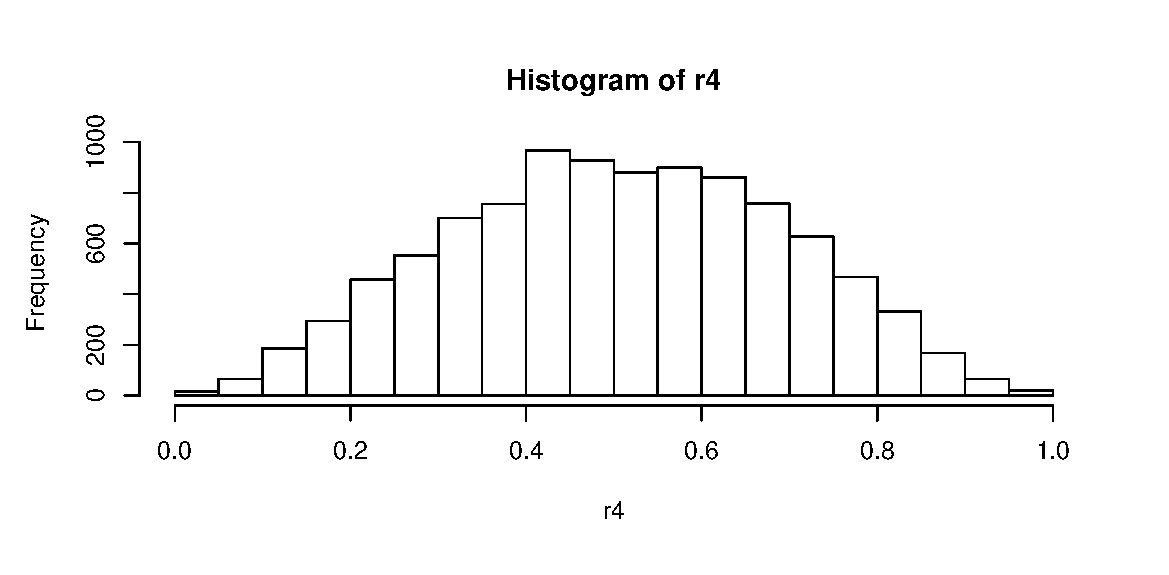
\includegraphics[width = 15cm]{r4.eps}
\caption{The numerical exp. of p4.}
\label{p4}
\end{figure}
\subsection{Analysis the efficiency}
As is mentioned in the PPT, the average number of iterations is c = 30/16. \\
However, if we generate Y first, which have a distribution $g(y) = 3y^2$, using the inverse transform algorithm, then c could be increased to 10, which means the average number of iteration is 10.
\end{proof}

\begin{problem}{5}
\text{ } \\
Use rejection method to generate a random variable with the distribution given.
\end{problem}
\begin{proof}
Let Y be a random variable with a distribution $g(x) = \lambda e^{-\lambda x}$. \\
Let $$h(x) = \frac{f(x)}{g(x)} = \frac{x^{2}e^{-x}}{2\lambda e^{-\lambda x}}.$$ 
Then $$\frac{dh(x)}{dx} = \frac{1}{2\lambda}e^{(\lambda-1)x}(2x+(\lambda-1)x^2).$$
We have $\frac{dh(x)}{dx} = 0$ when x = 0 or $x = \frac{2}{1-\lambda}$, provided that $\lambda < 1.$
% As $$\frac{d^{2}(h(x))}{dx^{2}} = \frac{1}{2\lambda}e^{(\lambda-1)x}((\lambda-1)^{2}x^{2} + 4(\lambda-1)x+2)$$
Hence $$c = max(h(x)) = h(\frac{2}{1-\lambda}) = \frac{2}{\lambda(1-\lambda)^{2}}e^{-2}.$$
Moreover, so as to minimize $c = c(\lambda)$, we should maximize $\lambda(1-\lambda)^{2}$.
As $\lambda(1-\lambda)^{2} = \frac{1}{2}*2\lambda(1-\lambda)(1-\lambda)\leqslant \frac{1}{2}(\frac{2\lambda + 2(1-\lambda)}{3})^{3} = \frac{4}{27},$ and it equals only when $2\lambda = 1-\lambda.$
In conclusion, the best $\lambda = \frac{1}{3}$, and c = $\frac{27}{2}e^{-2}$.
\subsection{The algorithm is as follows.}
-1. Set $c = \frac{2}{\lambda(1-\lambda)^{2}}e^{-2}.$ \\
0. While True: \\
1. Generate a random number U, set $Y = -\frac{1}{\lambda}log(U).$ \\
2. Generate a random number V.
3. if $V < \frac{f(Y)}{cg(Y)}$, set X = Y, RETURN.

\subsection{Numerical Experiment}
\subsubsection{The code is shown as follows}
\begin{lstlisting}[language = {R}]
# Problem 5
p5 = function(a, lambda) {
  f = function(x) {
    return(0.5 * x^2 *exp(-x))
  }
  g = function(x) {
    return(lambda * exp(-lambda * x))
  }
  c = 2/(lambda * (1-lambda)^2) * exp(-2)
  A = matrix(rep(0, a[1] * a[2]), ncol = a[2])
  for(i in 1:a[1]) {
    for(j in 1:a[2]) {
      while(1) {
        u = runif(1)
        y = -1/lambda * log(u)
        v = runif(1)
        if(v < f(y)/(c*g(y))) {
          A[i, j] = y
          break
        }
      }
    }
  }
  return(A)
}

# Problem 5
r5 = p5(a, lambda = 0.5)
hist(r5)
\end{lstlisting}
\subsubsection{The result is shown as follows}
\begin{figure}[htbp]
\centering
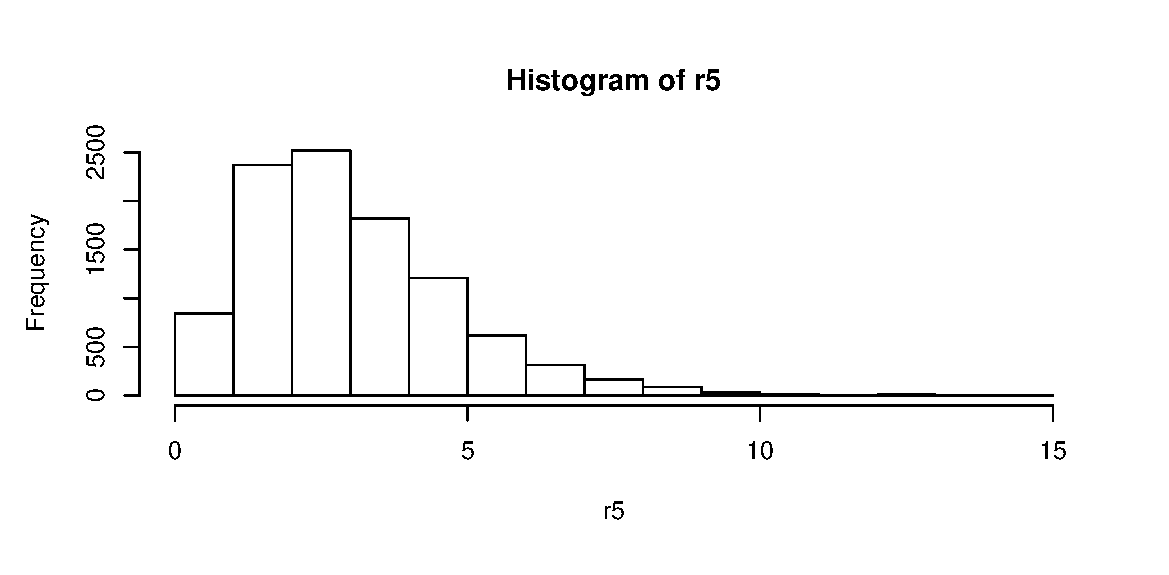
\includegraphics[width = 15cm]{r5.eps}
\caption{The numerical exp. of p5.}
\label{p5}
\end{figure}
\end{proof}

\end{document}
